
\begin{frame}[plain,c]
\begin{center}
{\Huge \bf Optional reading for Lecture \thislecture}
\end{center}
\end{frame}

% ------------------------------------------------------------------------------
% ------------------------------------------------------------------------------

%
% Worked example :
%

{
\problemslide

%
%
%

\begin{frame}{Worked example: Wire loop falling in magnetic field}

  \begin{blockexmplque}{Question}
    A rectangular loop of wire with dimensions $\ell$ and $w$ is released at
    $t=0$ from rest, just above a region in which the magnetic field is
    $\vec{B}_0$, as shown in the figure below.
    $\vec{B}_0$ is perpendicular to the loop of wire.
    \begin{center}
         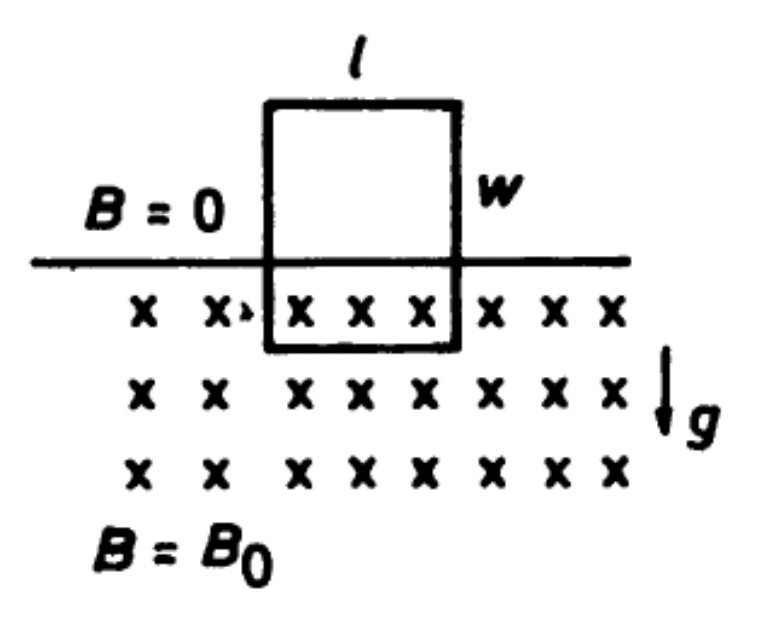
\includegraphics[width=0.35\textwidth]{./images/problems/lect11_wire_loop_falling_in_b_field}
     \end{center}
    The loop has resistance $R$, self-inductance $L$, and mass $m$.
    Consider the loop during the time that it has its upper edge
    in the zero-field region.\\
  \end{blockexmplque}

\end{frame}

%
%
%

\begin{frame}{Worked example: Wire loop falling in magnetic field}

  \begin{blockexmplque}{Question (cont'd)}
    \begin{itemize}
      \item
      Discuss the forces acting on the loop and write
      Newton’s equation of motion for the loop.
      \item
      Find expressions for the electromotive force induced by the motion
      of the loop in the magnetic field, as well as for the voltage drops
      due to the resistance and self-inductance of the loop and relate
      them via Kirchhoff’s voltage law.
      \item
      Assuming that you can ignore the self-inductance of the loop
      but not the resistance,
      find the current and velocity of the loop as functions of time.
      \item
      Assuming that you can ignore the resistance of the loop
      but not the self-inductance,
      find the current and velocity of the loop as functions of time.
    \end{itemize}
  \end{blockexmplque}

\end{frame}

%
%
%

\begin{frame}{Worked example: Wire loop falling in magnetic field}

  %
  % %%% 1
  %

  The loop has mass $m$ and the gravitational force that
  will be exerted upon would be:
  \begin{equation*}
    F_{g} = mg
  \end{equation*}

  At $t$=0, the horizontal (bottom) segment of the loop
  enters the magnetic field. At $t>0$, the magnetic force exerted
  upon that segment is given by:
  \begin{equation*}
    |\vec{F}_{B}| = | I \int_{\ell} d\vec{\ell} \times B | = B_0 \ell I
  \end{equation*}

  The magnetic force will point upwards and will oppose the
  gravitational force with points downwards.\\
  \vspace{0.2cm}

  Newton's law of motion for the loop is:
  \begin{equation*}
    mg - B_0 \ell I = m \frac{du}{dt}
  \end{equation*}

\end{frame}

%
%
%

\begin{frame}{Worked example: Wire loop falling in magnetic field}

  %
  % %%% 1
  %

  The electromotive force (EMF) that will be developed along the
  horizontal (bottom) segment of the loop is:
  \begin{equation*}
    \varepsilon =
      |\int_{\ell} (\vec{u} \times \vec{B}) \cdot d\vec{\ell}| = B_0 \ell u
  \end{equation*}

  The back-EMF due to the inductance L of the loop is:
  \begin{equation*}
    \varepsilon_{back} = V_{L} = - L \frac{dI}{dt}
  \end{equation*}

  The voltage drop due to the resistance R of the loop is:
  \begin{equation*}
    V_{R} = RI
  \end{equation*}

  Kirchoff's voltage law relates the directed sum of EMFs
  with the sum of voltage drops along the loop
  \begin{equation*}
    \varepsilon + \varepsilon_{back} = V_{R} \Rightarrow
    B_0 \ell u - L \frac{dI}{dt} = RI
  \end{equation*}

\end{frame}

%
%
%

\begin{frame}{Worked example: Wire loop falling in magnetic field}

  %
  % %%% 3
  %
  Assuming that $L=0$, Kirchoff's voltage law
  relates $I$ and $u$ as follows:
  \begin{equation*}
    B_0 \ell u - \cancelto{0}{L} \;\; \frac{dI}{dt} = RI \Rightarrow
    B_0 \ell u = RI \Rightarrow I = \frac{B_0 \ell}{R} u
  \end{equation*}

  Substituting the above expression for $I$
  in Newton's law yields:
  \begin{equation*}
    mg - B_0 \ell \Big( \frac{B_0 \ell}{R} u \Big) = m \frac{du}{dt} \Rightarrow
    \frac{du}{dt} = g - \frac{B_0^2 \ell^2}{mR} u \Rightarrow
  \end{equation*}
  \begin{equation*}
    \frac{d(u/g)}{dt} = 1 - \frac{B_0^2 \ell^2}{mR} (u/g)
  \end{equation*}

  By making the following substitutions:
  \begin{equation*}
    C = \frac{B_0^2 \ell^2}{mR} \;\;\; and \;\;\; u^{\prime} = u/g
  \end{equation*}

  the previous differential equation simplifies to:
  \begin{equation*}
    \frac{du^{\prime}}{dt} = 1 - C u^{\prime}
    \label{eq:p3c_u_diffeq2}
  \end{equation*}

\end{frame}

%
%
%

\begin{frame}{Worked example: Wire loop falling in magnetic field}

  Solving that differential equation:
  \begin{equation*}
    \frac{du^{\prime}}{1-Cu^{\prime}} = dt \Rightarrow
   -\frac{1}{C} \frac{d(1-Cu^{\prime})}{1-Cu^{\prime}} = dt \Rightarrow
  \end{equation*}

  \begin{equation*}
    \int_{u^{\prime}(t=0)=0}^{u^{\prime}(t>0)}
      \frac{d(1-Cu^{\prime})}{1-Cu^{\prime}} =
     -C \int_{\tau=0}^{\tau=t} d\tau \Rightarrow
   \end{equation*}
   \begin{equation*}
      ln\Big(1-Cu^{\prime}\Big) \Bigg\rvert_{0}^{u^{\prime}(t)}
      = -C \tau \Bigg\rvert_{0}^{t} \Rightarrow
  \end{equation*}

  \begin{equation*}
    ln\Big(1-Cu^{\prime}(t)\Big) - \cancelto{0}{ln(1)} = -C t \Rightarrow
  \end{equation*}

  \begin{equation*}
    1-Cu^{\prime}(t) = e^{-Ct} \Rightarrow
  \end{equation*}

  \begin{equation*}
    u^{\prime}(t) = \frac{1}{C} \Big( 1-e^{-Ct} \Big)
  \end{equation*}

\end{frame}

%
%
%

\begin{frame}{Worked example: Wire loop falling in magnetic field}

  Replacing $C$ and $u^\prime$ with their definitions, the above equation yields
  the sought after expression for $u$ as a function of time:
  \begin{equation*}
    u(t)/g =
     \frac{mR}{B_0^2 \ell^2} \Big( 1-e^{-\frac{B_0^2 \ell^2}{mR} t} \Big)
     \Rightarrow
  \end{equation*}

  \begin{equation*}
    u(t) =
     \frac{mgR}{B_0^2 \ell^2} \Big( 1-e^{-\frac{B_0^2 \ell^2}{mR} t} \Big)
  \end{equation*}

  Finally, substituting the above expression for $u(t)$, in the expression
  that resulted from Kirchoff's voltage law (relating $I$ and $u$), we find:
  \begin{equation*}
    I(t) = \frac{B_0 \ell}{R}
      \frac{mgR}{B_0^2 \ell^2} \Big( 1-e^{-\frac{B_0^2 \ell^2}{mR} t} \Big)
        \Rightarrow
  \end{equation*}
  \begin{equation*}
    I(t) = \frac{mg}{B_0 \ell} \Big( 1-e^{-\frac{B_0^2 \ell^2}{mR} t} \Big)
  \end{equation*}

\end{frame}

%
%
%

\begin{frame}{Worked example: Wire loop falling in magnetic field}

  %
  % %%% 4
  %

  Assuming that $R=0$, Kirchoff's voltage law
  relates $I$ and $u$ as follows:
  \begin{equation*}
    B_0 \ell u - L \frac{dI}{dt} = \cancelto{0}{R} \;\; I \Rightarrow
    B_0 \ell u = L \frac{dI}{dt} \Rightarrow
    \frac{dI}{dt} = \frac{B_0 \ell}{L} u
  \end{equation*}

  Differentiating with respect to time
  both sides of the previous expression of Newton's law of motion, yields:
  \begin{equation*}
    -B_0 \ell \frac{dI}{dt} = m \frac{d^2 u}{dt^2}
  \end{equation*}

  Combining the two expressions above, we find:
  \begin{equation*}
    -B_0 \ell \Big( \frac{B_0 \ell}{L} u \Big) = m \frac{d^2 u}{dt^2} \Rightarrow
    -\frac{B_0^2 \ell^2}{L} u = m \frac{d^2 u}{dt^2} \Rightarrow
  \end{equation*}

  \begin{equation*}
    \frac{d^2 u}{dt^2} + \frac{B_0^2 \ell^2}{mL} u = 0
  \end{equation*}

\end{frame}

%
%
%

\begin{frame}{Worked example: Wire loop falling in magnetic field}

  Making the following substitution:
  \begin{equation*}
    \omega^2 = \frac{B_0^2 \ell^2}{mL}
  \end{equation*}

  the previous above differential equation becomes:
  \begin{equation*}
    \frac{d^2 u}{dt^2} + \omega^2 u = 0
  \end{equation*}

  This is the well-known differential equation for the harmonic oscillator
  that has solutions of the form:
  \begin{equation*}
    u(t) = a_1 cos(\omega t) + a_2 sin(\omega t)
  \end{equation*}
  where $a_1$ and $a_2$ are determined from the given
  boundary conditions:
  \begin{equation*}
    u(t=0) = 0 \;\;\; \text{and} \;\;\; I(t=0) = 0
  \end{equation*}

\end{frame}

%
%
%

\begin{frame}{Worked example: Wire loop falling in magnetic field}

  The first of these boundary conditions yields:
  \begin{equation*}
    u(t=0) = a_1 \cancelto{1}{cos(0)} + a_2 \cancelto{0}{sin(0)} = a_1
    \Rightarrow
    a_1 = 0
  \end{equation*}
  Therefore, the general solution for $u(t)$ is reduced to:
  \begin{equation*}
    u(t) = a_2 sin(\omega t)
    \label{eq:p3d_ut_bc1}
  \end{equation*}

  From the expression of Newton's law of motion at $t=0$, we find:
  \begin{equation*}
    mg - B_0 \ell \cancelto{0}{I(0)} \; =
       m \frac{du}{dt} \Bigg\rvert_{t=0}
  \end{equation*}

  Substituting the above expression for $u(t)$, we have:
  \begin{equation*}
    \cancel{m}g =
       \cancel{m} \frac{d}{dt}
         \Big( a_2 sin(\omega t) \Big)\Bigg\rvert_{t=0} \Rightarrow
    g = a_2 \omega cos(\omega t)\Bigg\rvert_{t=0} \Rightarrow
    a_2 = \frac{g}{\omega}
  \end{equation*}

\end{frame}

%
%
%

\begin{frame}{Worked example: Wire loop falling in magnetic field}

  So, finally, the required expression for $u(t)$ is:
  \begin{equation*}
    u(t) = \frac{g}{\omega} sin(\omega t)
  \end{equation*}

  where $\omega$ is given by:
  \begin{equation*}
    \omega = \frac{B_0 \ell}{\sqrt{mL}}
  \end{equation*}

  To find the required expression for $I(t)$, we substitute the above
  exression for $u(t)$ in Kirchoff's voltage law:
  \begin{equation*}
    \frac{dI}{dt} =
     \frac{B_0 \ell}{L}
      \Big( \frac{g}{\omega} sin(\omega t) \Big) =
      \frac{B_0 \ell g}{L \omega} sin(\omega t)
  \end{equation*}

\end{frame}

%
%
%

\begin{frame}{Worked example: Wire loop falling in magnetic field}

  Solving this differential equation:
  \begin{equation*}
    \int_{I(0)}^{I(t)} dI =
     \frac{B_0 \ell g}{L \omega}
       \int_{0}^{t} sin(\omega t^\prime) dt^\prime \Rightarrow
  \end{equation*}

  \begin{equation*}
     I \Bigg\rvert_{I(0)}^{I(t)} =
      - \frac{B_0 \ell g}{L \omega^2}
          cos(\omega t^\prime) \Bigg\rvert_{0}^{t} \Rightarrow
     I(t) - \cancelto{0}{I(0)} \; =
      - \frac{B_0 \ell g}{L \omega^2}
        \Big( cos(\omega t) - 1 \Big)  \Rightarrow
  \end{equation*}

  \vspace{0.2cm}

  we find:
  \begin{equation*}
     I(t) =
        \frac{B_0 \ell g}{L \omega^2}
        \Big( 1 - cos(\omega t) \Big)
        \xRightarrow{\omega^2 = \frac{B_0^2 \ell^2}{mL}}
  \end{equation*}


  \begin{equation*}
     I(t) =
        \frac{mg}{B_0 \ell}
        \Big( 1 - cos(\omega t) \Big)
  \end{equation*}

\end{frame}

} % Worked example

% ------------------------------------------------------------------------------

%
% Worked example :
%

{
\problemslide

%
%
%

\begin{frame}{Worked example: Square loop midway two parallel wires}

  \begin{blockexmplque}{Question}
    A square loop of wire, of side $\alpha$, lies midway between
    two long wires, 3$\alpha$ apart, and in the same plane.
    The long wires are the sides of a large rectangular loop, but the short
    ends are so far away that they can be neglected.
    \begin{center}
     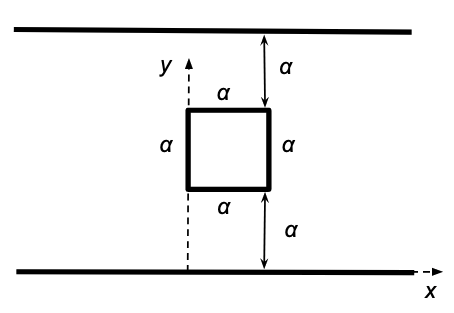
\includegraphics[width=0.55\textwidth]{./images/problems/lect11_square_loop_between_wires_2}\\
    \end{center}
 \end{blockexmplque}

\end{frame}

%
%
%

\begin{frame}{Worked example: Square loop midway two parallel wires}

  \begin{blockexmplque}{Question}
    If a steady, clockwise current $I$ circulates in the large loop:
    \begin{itemize}
    \item
    Determine an expression for the magnetic field $\vec{B}$\\
    in the region of the small loop.
    \item
    Calculate the magnetic flux through the small loop.
    \item
    Find an expression for the mutual inductance $M$\\
    of the system of two loops.
    \end{itemize}
   If, instead, a clockwise current $I$ circulates in the small loop, and\\
   assuming that this current is gradually increasing
   ($dI/dt = k > 0$,\\ where $k$ is a constant):
    \begin{itemize}
    \item
    Calculate the electromotive force induced in the large loop.
    \item
    Find the direction of the current induced in the large loop.
    \end{itemize}
  \end{blockexmplque}

 \end{frame}

 %
 %
 %

 \begin{frame}{Worked example: Square loop midway two parallel wires}

   % a
   The magnetic field $\vec{B}_{i}$ produced by a single,
   infinite straight wire $i$ with current $I_i$, is given by:
   \begin{equation*}
     \vec{B}_i = \frac{\mu_0 I_i}{2\pi r} \hat{\phi}
   \end{equation*}
   where $r$ is the distance from the wire.\\
   \vspace{0.2cm}

   The total magnetic field in the area of the small loop, will have contributions
   from each of the long wires of the big loop.\\
   \vspace{0.2cm}

   The superposition principle allows
   us to add these contributions due to single wires.\\
   \vspace{0.2cm}

   If the current $I$ in the big loop runs clockwisely,
   the direction of $\vec{B}$ is into the page (towards the negative $z$ axis).\\


\end{frame}

%
%
%

\begin{frame}{Worked example: Square loop midway two parallel wires}

   We can write the total field $\vec{B}$ in the area of the small loop as:
   \begin{equation*}
     \vec{B} = - \Big( \frac{\mu_0 I}{2\pi y} +
                       \frac{\mu_0 I}{2\pi (3\alpha-y)}
                  \Big) \hat{z}
             = - \frac{\mu_0 I}{2\pi}
                 \Big( \frac{1}{y} +
                       \frac{1}{3\alpha-y} \Big) \hat{z}
   \end{equation*}
   where $y$ is the distance from the bottom wire of the large loop.\\
   \vspace{0.2cm}

   %b

   The magnetic flux $\Phi$ through the small loop, is:
   \begin{equation*}
     \Phi = \int \vec{B} \cdot d\vec{S}
   \end{equation*}
   where $d\vec{S}$ is perpendicular to the small loop,
   and will be taken to point into the page (in the negative $z$ direction),
   in the same direction as $\vec{B}$.\\
   \vspace{0.2cm}

   Since the magnetic field $\vec{B}$ depends on $y$, but not the perpendicular
   direction $x$ on the plane of the small loop, we will write the
   element $d\vec{S}$ as:
   \begin{equation*}
     d\vec{S} = - x dy \hat{z}
   \end{equation*}

 \end{frame}

 %
 %
 %

 \begin{frame}{Worked example: Square loop midway two parallel wires}

   Substituting the above expressions for $\vec{B}$ and $d\vec{S}$ into the
   expression for $\Phi$, we have:

   \begin{equation*}
     \Phi = \frac{\mu_0 I}{2\pi}
             \int_{small\;loop}
               \Big( \frac{1}{y} +
                     \frac{1}{3\alpha-y} \Big) x dy =
           \frac{\mu_0 I \alpha}{2\pi}
           \int_{\alpha}^{2\alpha}
             \Big( \frac{1}{y} +
                   \frac{1}{3\alpha-x} \Big) dy
   \end{equation*}

   \vspace{0.3cm}

   Carrying out the integration over $x$, we find:
   \begin{equation*}
     \Phi = \frac{\mu_0 I \alpha}{2\pi}
            \int_{\alpha}^{2\alpha}
             \Big( \frac{1}{y} +
                   \frac{1}{3\alpha-y} \Big) dy
         = \frac{\mu_0 I \alpha}{2\pi}
             \Big( ln(y)\Big\rvert_{\alpha}^{2\alpha} -
                   ln(3\alpha-y)\Big\rvert_{\alpha}^{2\alpha} \Big) \Rightarrow
   \end{equation*}
   \begin{equation*}
     \Phi = \frac{\mu_0 I \alpha}{2\pi}
             \Big( ln(2\alpha) - ln(\alpha)
                 - ln(\alpha) + ln(2\alpha) \Big) \Rightarrow
   \end{equation*}
   \begin{equation*}
     \Phi = \frac{\mu_0 I \alpha ln2}{\pi}
   \end{equation*}

\end{frame}

 %
 %
 %

\begin{frame}{Worked example: Square loop midway two parallel wires}

   % c

   The mutual inductance $M$ of the system of two loops,
   connects the flux in one loop with the current in the other:
   \begin{equation*}
     \Phi = M I
   \end{equation*}

   Therefore, using the expression for $\Phi$ above:
   \begin{equation*}
     M = \frac{\mu_0 \alpha ln2}{\pi}
   \end{equation*}

   \vspace{0.2cm}

   % d

   If a clockwise current $I$ circulates in the small loop,
   the emf $\varepsilon$ induced in the big loop, is given by:
   \begin{equation*}
     \varepsilon = -\frac{d\Phi}{dt}
   \end{equation*}
   where $\Phi$ is the electric flux through that loop.

   The flux $\Phi$ is given by
   \begin{equation*}
     \Phi = M^\prime I
   \end{equation*}
   where $M^\prime$ is the mutual inductance of the two loops, and
   $I$ is the current on the small loop.

\end{frame}

  %
  %
  %

\begin{frame}{Worked example: Square loop midway two parallel wires}

   Previously, we calculated an expression for $M$, connecting the
   flux in the small loop with a current on the big loop.
   But $M^\prime = M$, so we can reuse the previous result for $M$:
   \begin{equation*}
     \varepsilon = -\frac{d\Phi}{dt} = -M \frac{dI}{dt} = -M k
   \end{equation*}
   Therefore, from the earlier expression for $\varepsilon$
   in the small loop, we find:
   \begin{equation*}
     \varepsilon = - \frac{\mu_0 \alpha k ln2}{\pi}
   \end{equation*}

   % e

   The net flux through the big loop, due to the current on the small loop,
   is into the page (The field lines point into the page, inside the small
   loop, and out of the page, outside the small loop. The big loop encloses
   all of the former, but only part of the latter, hence the net flux is
   into the page.\\
   \vspace{0.1cm}

   This flux is increasing ($dI/dt = k > 0$).\\
   \vspace{0.1cm}

   Therefore, the induced current in the big loop is such that its field
   points out of the page: It flows counterclockwise.\\

 \end{frame}

} % Worked example

% ------------------------------------------------------------------------------

%
% Worked example :
%

{
\problemslide

%
%
%

\begin{frame}{Worked example: Toroid with rectangular cross section}

  \begin{blockexmplque}{Question}
    A toroid has a rectangular cross section, as shown in the figure below.
    \begin{center}
     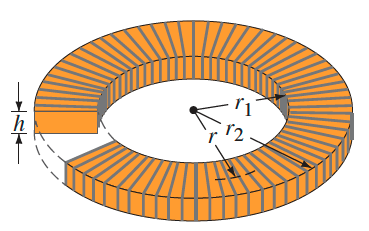
\includegraphics[width=0.40\textwidth]{./images/problems/lect11_toroid}\\
    \end{center}
    \vspace{-0.2cm}
    \begin{itemize}
      \item
      Show that the self-inductance is:
      \begin{equation*}
          L = \frac{\mu_0 N^2 h}{2\pi} ln\frac{r_2}{r_1}
      \end{equation*}
      where $N$ is the total number of turns and $r_1$, $r_2$ and $h$
      are the dimensions shown in the figure above.
    \end{itemize}
  \end{blockexmplque}

\end{frame}

%
%
%

\begin{frame}{Worked example: Toroid with rectangular cross section}

  \begin{blockexmplque}{Question}
    \begin{itemize}
      \item
      Determine the energy density in the magnetic field as a function of $r$
      ($r_1 < r < r_2$) and integrate this over the volume to obtain the total
      energy stored in the toroid, which carries a current $I$ in each
      of its $N$ loops.
    \end{itemize}
  \end{blockexmplque}

  The self-inductance $L$ connects the magnetic flux linkage $N\Phi_B$
  and the current in the toroidal coil:
  \begin{equation*}
    N\Phi_B = L I
  \end{equation*}

  Therefore:
  \begin{equation*}
    L = \frac{N\Phi_B}{I}
  \end{equation*}

  $\Phi_B$ is the magnetic flux through a single turn (out of the $N$ turns
  in the coil) and it is given by:
  \begin{equation*}
    \Phi_B = \int_{single\;\;turn}\vec{B} \cdot d\vec{S}
  \end{equation*}

\end{frame}

%
%
%

\begin{frame}{Worked example: Toroid with rectangular cross section}

  The magnetic field or the toroid can be computed from Ampere's law:
  \begin{equation*}
    \oint_{L} \vec{B} \cdot d\vec{\ell} = \mu_0 I_{encl}
  \end{equation*}
  If $L$ is a circular path with radius $r$, concentric with the toroid,
  then the symmetry of the problem suggests that:
  \begin{equation*}
    B 2\pi r = \mu_0 I_{encl} \xRightarrow{I_{encl} = NI}
    B 2\pi r = \mu_0 NI \Rightarrow
    B = \frac{\mu_0 NI}{2\pi r}
  \end{equation*}
  The magnetic field is azimuthal and in vector form can be written as:
  \begin{equation*}
    \vec{B} = \frac{\mu_0 NI}{2\pi r} \hat{\phi}
  \end{equation*}

  Using the above expression for $B$, the flux $\Phi_B$ becomes:
  \begin{equation*}
    \Phi_B = \int_{single\;\;turn} \Big( \frac{\mu_0 NI}{2\pi r} \hat{\phi} \Big) \cdot d\vec{S}
           = \frac{\mu_0 NI}{2\pi} \int_{single\;\;turn} \Big( \frac{1}{r} \hat{\phi} \Big) \cdot d\vec{S}
  \end{equation*}

\end{frame}

%
%
%

\begin{frame}{Worked example: Toroid with rectangular cross section}

  The surface element $d\vec{S}$ on a single turn of the toroid
  can be expressed as:
  \begin{equation*}
    d\vec{S} = h dr \hat{\phi}
  \end{equation*}
  The expession for $\Phi_B$ yields:
  \begin{equation*}
    \Phi_B = \frac{\mu_0 NI}{2\pi} \int_{single\;\;turn} \Big( \frac{1}{r} \hat{\phi} \Big) \cdot \Big( h dr \hat{\phi} \Big)
           = \frac{\mu_0 NI h}{2\pi} \int_{r_1}^{r_2} \frac{dr}{r} \Rightarrow
  \end{equation*}
  \begin{equation*}
    \Phi_B = \frac{\mu_0 NI h}{2\pi} ln(\frac{r_2}{r_1})
  \end{equation*}

  Therefore, the earlier expressed for the self-inductance $L$ can be written as:
  \begin{equation*}
    L = \frac{N}{I} \Big( \frac{\mu_0 NI h}{2\pi} ln(\frac{r_2}{r_1}) \Big)
      = \frac{\mu_0 N^2 h}{2\pi} ln(\frac{r_2}{r_1})
  \end{equation*}

\end{frame}

%
%
%

\begin{frame}{Worked example: Toroid with rectangular cross section}

  The energy density $u_B$ in the magnetic field is given by:
  \begin{equation*}
    u_B = \frac{1}{2\mu_0} B^2
  \end{equation*}

  Subsituting the expression for $B$ in the toroidal coil, we find:
  \begin{equation*}
    u_B = \frac{1}{2\mu_0} \Big( \frac{\mu_0 NI}{2\pi r} \Big)^2
        = \frac{\mu_0 N^2 I^2}{8\pi^2 r^2}
  \end{equation*}

  The total energy $U_B$ stored in the magnetic field is given by:
  \begin{equation*}
    U_B = \int_{coil\;\;volume} u_B d\tau
  \end{equation*}

  Substituting the expression for $u_B$, the above yields:
  \begin{equation*}
    U_B = \int_{coil\;\;volume} \frac{\mu_0 N^2 I^2}{8\pi^2 r^2} d\tau
        = \frac{\mu_0 N^2 I^2}{8\pi^2} \int_{coil\;\;volume} \frac{1}{r^2} d\tau
  \end{equation*}

\end{frame}

%
%
%

\begin{frame}{Worked example: Toroid with rectangular cross section}

  The volume element $d\tau$ within the coil, considering that the integrand
  above depends only on $r$, can be written as:
  \begin{equation*}
    d\tau = h 2\pi r dr
  \end{equation*}

  Therefore:
  \begin{equation*}
    U_B = \frac{\mu_0 N^2 I^2}{8\pi^2} \int_{coil\;\;volume} \frac{1}{r^2} h 2\pi r dr
        = \frac{\mu_0 N^2 I^2 h}{4\pi} \int_{r_1}^{r_2} \frac{dr}{r} \Rightarrow
  \end{equation*}
  \begin{equation*}
    U_B = \frac{\mu_0 N^2 I^2 h}{4\pi} ln(\frac{r_2}{r_1})
  \end{equation*}

\end{frame}

} % Worked example
